\documentclass[journal]{./IEEE/IEEEtran}
\usepackage{cite,graphicx}

\newcommand{\SPTITLE}{Text Prediction using Probability Matrices and Prefix Trees}
\newcommand{\ADVISEE}{John Alvin L. Sayson}
\newcommand{\ADVISER}{Fermin Roberto G. Lapitan}

\newcommand{\BSCS}{Bachelor of Science in Computer Science}
\newcommand{\ICS}{Institute of Computer Science}
\newcommand{\UPLB}{University of the Philippines Los Ba\~{n}os}
\newcommand{\REMARK}{\thanks{Presented to the Faculty of the \ICS, \UPLB\
                             in partial fulfillment of the requirements
                             for the Degree of \BSCS}}
        
\markboth{CMSC 190 Special Problem, \ICS}{}
\title{\SPTITLE}
\author{\ADVISEE~and~\ADVISER
\REMARK
}
\pubid{\copyright~2019~ICS \UPLB}

%%%%%%%%%%%%%%%%%%%%%%%%%%%%%%%%%%%%%%%%%%%%%%%%%%%%%%%%%%%%%%%%%%%%%%%%%%

\begin{document}

% TITLE
\maketitle

% ABSTRACT
\begin{abstract}
With the advent of the digital age, communication has evolved to a point where technology is seamlessly integrated into day-to-day conversation. Primarily found in mobile phones, text prediction systems involves streamlining the communication by providing users with suggested words that they can select, based on the previous word they provided. This study aims to implement a similar technology, embedded in an application developed for the Chrome browser to provide the power of text prediction in desktop environments, in an application most users use in their day-to-day lives. The predictor was developed using various representations of the text input, where probability matrices and prefix trees provide the most importance.
\end{abstract}

% INDEX TERMS
\begin{keywords}
text generation, text prediction, probability matrices, prefix trees
\end{keywords}

% INTRODUCTION
\section{Introduction}
Verbal communication was always been a vital component of human interaction. After all, it allows two people to be able to understand each other. With the influx and rapid growth of technology over the previous decades, new methods of communication in the digital age were conceived over that timespan.

Nowadays, prediction keyboards are commonplace in mobile phones. Numerous mobile operating systems seamlessly integrate prediction into the existing keyboard functions to the point where people use it switching from the regular keyboard, to the prediction keyboard, and back again.

It might be common in mobile systems, but what about desktop ones? This study involved investigation on two online applications that provide generated outputs from predefined inputs.

AIWriter\cite{AIWriter} and Botnik's Voicebox\cite{Voicebox} are these two applications. AIWriter's process is fully automatic, instantly generating works depending on settings provided by the user in the beginning. On the other hand, Voicebox is more of a hands-on process as the user selects the words suggested by the application in writing their literary works. The suggested words are determined by the source text the user selected in the beginning, ranging from Harry Potter narrations to pancake recipes. If the selection range does not interest the user, they can provide their own source texts by uploading it to the website.

Both website applications improve writing time by doing away with manual word-for-word typing, providing either words or complete paragraphs for the users to use right away. This study intends to provide a similar convenience.

For those with cognitive, perceptive, and/or physical disabilities, predictive text systems were their preferred medium in being able to communicate easier in social settings. \cite{GV2006} Being able to just use one tap to select words rather than multiple taps per letter, it allows for a great increase in convenience when it comes to conversation. Over time, continuous usage of these systems can further personalize the suggested words to the user. Through this, the rate of communication between people can improve even further. This application aims to achieve a similar goal to that of the common predictive text system. By providing an interface wherein users are given suggestions while in the middle of creating texts, they are able to utilize the power of mobile prediction keyboard functionalities.

The application that was implemented as the main output of this study differs from the aforementioned Voicebox in the way the initial input is accepted. The application accepts user input as the initial data for the probability matrix and a prefix tree, which are the two main data structures used for the application.

This paper shall discuss the implementation for the text prediction, as well as the application interface for it.

Generally, the study aims to create a text prediction model that utilizes a probability matrix and a prefix tree as its data structures.

On a more specific standpoint the study aims to achieve the following:
\begin{enumerate}{\setlabelwidth{1.}}

\item[1.] Produce a sequence and bag-of-words representation of input in order to create the probability matrix and prefix tree;

\item[2.] Create an application that will allow a user to interact with an instance of the text prediction model; and

\item[3.] Assess the application created and the perceived accuracy of the two levels of prediction through surveys.

\end{enumerate}

The inputs for the application only considered text that is typed using the default browser encoding. As such, languages that do not use this encoding are not part of this study's scope.

% RRL
\section{Review of Related Literature}

%ACTUAL CONTENT OF RRL
To understand the possible applications and previous implementations of story and text generation, previous works in the field were observed.
\pubidadjcol

%\subsection{Previous Advances in Text and Literary Work Generation}
%Online Works
%Text Generation from Keywords
Uchimoto, et al. presented various text-generation models in their paper wherein Japanese sentences are formed by feeding the program keywords which serve as the subjects of the sentence it produces. \cite{UKIHSS2002} 
%Discuss some of the language models...

A table of input-output pairs were provided by the authors, with inputs being words in groups of threes and the outputs being complete sentences. From this, a possible limitation provided by their application was that it could only accept three inputs at a time.

The authors have mentioned that the program was created for speakers that are not as fluent in Japanese be able to express sentences that they intend to speak but only know the main words that they want to express. This shows that text generation is not limited to recreational applications, and can be used for accessibility and elaboration. %continue...

%Chinese Poetry Generation with Recurrent Neural Networks
X. Zhang and M. Lapata utilized recurrent neural networks in 2014 to generate Chinese poetry, which follows a specific format for it to be considered one.
\cite{ZXLM2014}
The Chinese poems that they generated follow the quatrain format, wherein four lines of poetry must have five or seven characters each.
The poetry generator functions similarly to Uchimoto's 2002 paper where keywords are accepted to outline the poem's main concept.
In creating the first line, a language model is used to rank candidates that satisfies criteria defined by the poetry format. Following lines are then based on the previous lines. This will ensure continuity from the first line to the last.

Text generation has also ventured into literary fields with less constraints, specifically story writing.

In 2018, A. Fan, et al. added sentence prompt generation (aside from the expected story generation component) which was then based on to create the corresponding stories. \cite{FLD2018} These prompts are created using a convolutional language model, which contains a novel gated self-attention mechanism created by some of the authors. \cite{DFAG2016}
They also used a sequence-to-sequence network, a model that uses two recurrent neural networks as encoders and decoders, to generate the story based on the prompts trained on the convolutional language model. The sequence-to-sequence model depended upon the trained prompts from the convolutional language model, resulting in a fusion model, as referred to by the writers.

Results shown in the paper contained comparisons between the fusion model and another language model,  presenting the former's readability and higher quality of output over the latter. However, the authors mentioned that one of the limitations of the fusion model is the genericness of the prompts generated, compared to human prompts. This limits the results that can be generated as more specific and varied prompts can provide better results.

% METHODOLOGY
\section {Methodology}
This section contains the technologies used in implementing the application, as well as a detailed look into the data structures used and the program flow of the model.

\subsection{Technologies Used}
The application was implemented using only JavaScript, along with the Chrome Extension API to integrate the application with the browser. Java was used to clean and slice a text input from a file. The output was then used in another version of the resulting application (which is discussed in a later section).

\subsection{Text Input Representations}
\subsubsection{Sequence}
The sequence is a simple array of strings from the input text, split by a single space (" ") delimiter.

\subsubsection{Bag-of-Words}
The bag-of-words then uses this sequence to count word occurrences.

\subsubsection{Probability Matrix}
The probability matrix uses both previously mentioned representations to produce the probability of a word to appear given another word. This is represented as the matrix keys, which is obtained from the keys of the bag-of-words.

\subsubsection{Prefix Tree}
The prefix tree uses the sequence representation to create the network of letters.

\subsection{Program Flow}
\begin{figure}[!ht]
\begin{center}

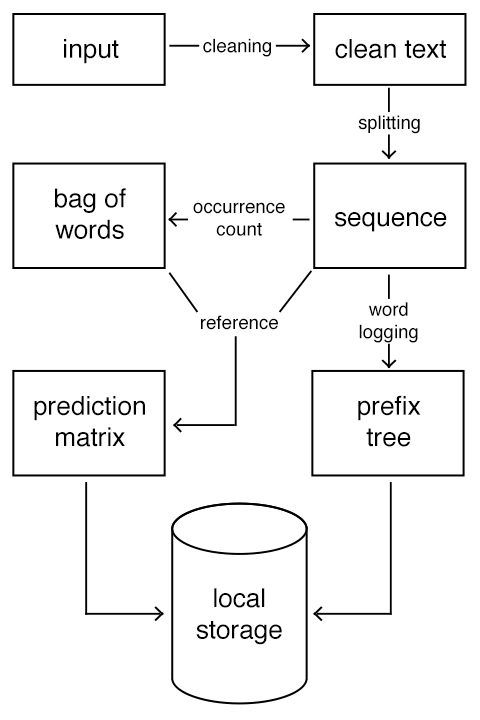
\includegraphics[width=65mm]{images/model.jpg}
\caption{The model used in implementing the predictor.}

\end{center}
\end{figure}

Fig. 1 illustrates the model used in the application, which shall be explained in this section.

\subsubsection{Input}
Upon installation of the extension, preliminary input data is accepted in a HTML page where the user is asked to enter it. The prefix tree is also loaded with the top 100 common words (according to the Oxford English Corpus) \cite{OxfordFacts}, along with the words provided by the user.

\subsubsection{Processing}
Upon selection of the [Begin Predicting] button in the page for the newly-installed extension, these words are then converted into the four representations mentioned earlier.

Before producing these representations of the text, the text is first cleaned in order to remove various characters and long spaces, which is vital for creating the sequence.

The created matrix and prefix tree is stored in the local storage of the browser. The bag-of-words and sequence representations are stored inside the matrix as reference.

In the Text Entry page, clicking on either Update Predictor, Copy to Clipboard, or Cast to Text Button converts the new input into the four representations. However, instead of directly storing it in the local storage, the application retrieves the saved matrix and prefix tree and merges it with the new ones.

\subsubsection{Output}
While typing in the available text box in the Text Entry Page, the caret location in said text box is used in determining the level of prediction for the next word. If the previously typed word has a space after it, it performs word-level prediction. Else, it performs letter-level prediction.

Word-level prediction uses the matrix, while letter-level prediction uses the prefix tree.

Determining results from the letter-level prediction involves navigating the tree for each letter of the word to be searched and then adding all results from that point onward into an array. It stops storing words when the size of the array reaches its maximum size (which is denoted by the number of keywords in the Settings page).

For word-level prediction, the class NameProbabilityPair is used in arranging the most probable words by percentage. Determining the values for the NameProbabilityPair is defined using the equation from the Bayes' theorem, where A is the word to generate possible outputs from, and B is one of the candidate words:
$$ P(A \mid B) = \frac{P(B \mid A) \, P(A)}{P(B)} $$

Meanwhile, the probability of a word is given by this equation:
$$ P(A) = \frac{count(A)}{count(total)} $$

The product of the two are then divided by the probability of B, obtained the same way as A.

The NameProbabilityPairs are stored in an array. This array is sorted after every word checked. When this array exceeds the number defined by the user in Settings, the least ranking entry is removed in order to maintain the number of words returned.

The results from these predictions are displayed on the area below the text box, the number which is defined by the user in Settings (default is 6). When these results are clicked, the application begins to look again for the possible words that come after it.

\section{Results and Discussion}
This section shall discuss the resulting interface, as well as the evaluation results.

\subsection{Interface}
The application consists of three main screens, the New Predictor screen, the Text Entry screen, and the Settings screen.

\subsubsection{New Predictor}
This screen appears when the extension is installed or upon reset of the predictor.

\begin{figure}[!ht]
\begin{center}

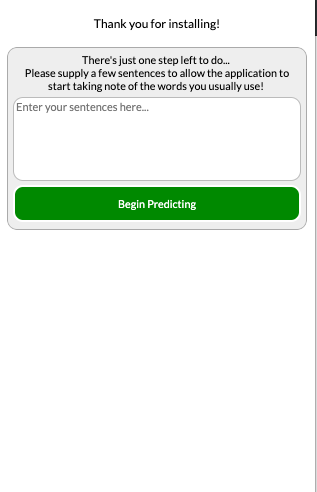
\includegraphics[width=65mm]{images/initial-input.png}
\caption{The New Predictor screen with input.}

\end{center}
\end{figure}

\subsubsection{Text Entry}
This screen appears after the initial state of the predictor has been created and saved to the local storage. This screen features four major functionalities: Update Predictor, Copy to Clipboard, Cast to Text Box, and Clear.

When the Update Predictor button is clicked, the words in the text box are stored into the probability matrix and the prefix tree,

Clicking on Copy to Clipboard does what the Update Predictor functionality does, and then it stores the text in the text box to the clipboard for pasting.

Before clicking on the Cast to Text Box button, the user must have first clicked on a text box in the website they are currently on. The application accepts a few types of valid text boxes for casting: textarea elements, and input elements with types "text" and "search". After satisfying the prerequisite, clicking the button updates the predictor and places the text on the popup's text box to the text box in the website.

\begin{figure}[!ht]
\begin{center}

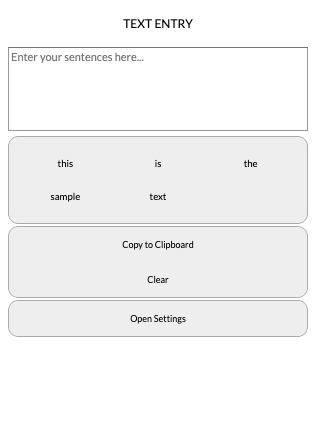
\includegraphics[width=65mm]{images/initial-text-entry.png}
\caption{The Text Entry screen with posted results based off of the input in the previous screen.}

\end{center}
\end{figure}

Fig. 4 illustrates the word-level prediction for the previous input, which is the word "this". On the other hand, Fig. 5 showcases the letter-level prediction functionality in the application with the input "a".

\begin{figure}[!ht]
\begin{center}

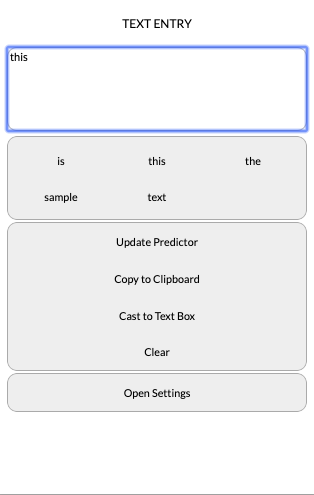
\includegraphics[width=65mm]{images/word-level-prediction.png}
\caption{Word-level prediction functionality.}

\end{center}
\end{figure}

\begin{figure}[!ht]
\begin{center}

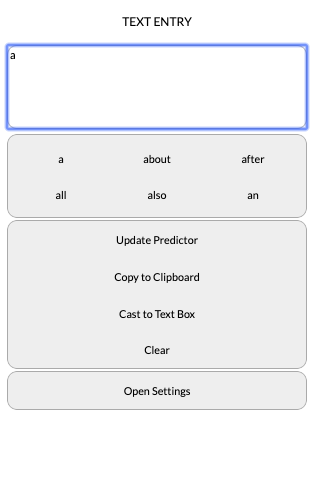
\includegraphics[width=65mm]{images/letter-level-prediction.png}
\caption{Letter-level prediction functionality.}

\end{center}
\end{figure}

\subsubsection{Settings}
Clicking the Open Settings button in the Text Entry loads this screen. This contains the slider for the number of keywords that will appear on the Text Entry, as well as the option to reset the application to its initial state.

\begin{figure}[!ht]
\begin{center}

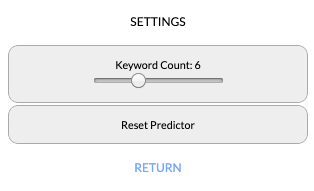
\includegraphics[width=65mm]{images/settings.png}
\caption{The Settings screen.}

\end{center}
\end{figure}

\subsection{Application Evaluation}
The application was evaluated through a survey answered by twenty people selected at random, using the System Usability Scale as a guide (with small modifications for the statements to fit the context of the study). The respondents were to rate the statements provided by the survey from a 1-5, where 1 means that they completely disagree with the statement and 5 for the opposite.

The application provided for testing consists of two versions. One version of the application is only preloaded with the most common 100 words in the English language, and the other was preloaded with a passage of the book \textit{Harry Potter and the Philosopher's Stone}. This was done in order to compare user satisfaction from a newly installed version of the application versus another version where it simulates the performance of the application when it has been used for a longer time. These versions shall be called S (for small) and L (for large), respectively.

The following is a list of the survey questions based from the System Usability Scale\cite{UsabilityGeeks}:

\begin{enumerate}{\setlabelwidth{1.}}

\item[1.] I think that I would like to use the application frequently.

\item[2.] I found the application unnecessarily complex.

\item[3.] I thought the application was easy to use.

\item[4.] I think that I would need the support of a technical person to be able to use this application.

\item[5.] I found the various functions in this application were well integrated.

\item[6.] I thought there was too much inconsistency in this application.

\item[7.] I would imagine that most people would learn to use this application very quickly.

\item[8.] I found the application very cumbersome to use.

\item[9.] I felt very confident using the application.

\item[10.] I needed to learn a lot of things before I could get going with this application.

\end{enumerate}

Getting a score from the SUS consists of the following steps, according to the same source:

\begin{enumerate}{\setlabelwidth{1.}}

\item[1.] Subtract 1 from the scores on all odd-numbered statements.

\item[2.] Subtract the score from 5 for all even-numbered statements.

\item[3.] Get the total for all numbers, and multiply it by 2.5.

\end{enumerate}

These steps were followed to compute the score for each individual response, and those were averaged to obtain the scores for both versions. The resulting score of the L version was 75.8, while the S version had a score of 76.9. According to the source, these scores are below a grade of A (which is a score of 80.3), and above a grade of C (which is a score of 68).

Aside from the questions derived from the System Usability Scale's template, two more were added to evaluate the user's perceived accuracy of the word- and letter-level prediction functionality of the application. This also followed the 1-5 rating scale of the previous ten questions.

\begin{enumerate}{\setlabelwidth{1.}}

\item[1.] I think that the word-level prediction for the application provides me with results I expect to appear.

\item[2.] I think that the letter-level prediction for the application provides me with results I expect to appear.

\end{enumerate}

As these two statements are not part of the System Usability Scale score computation, only the weighted average of the responses was used in comparing the two versions.

The L version obtained the scores 4.4 and 4.3 for word- and level-letter level predictions respectively, while the S version obtained 4.45 and 4.25. It is worth noting that the S version was perceived to be more accurate than the L version with regards to word-level prediction, while the opposite was true for letter-level prediction.

% CONCLUSION AND FUTURE WORK
\section{Conclusion and Future Work}
This study was able to create a text prediction model implemented using a probability matrix and a prefix tree, as well as sequences and bags-of-words. Through its evaluation as an application for the Chrome browser, it was able to obtain satisfactory results with regards to perceived accuracy and the usability of the application itself.

The model does not perform optimization as the probability matrix and the prefix tree grows bigger with each user input. Future studies can look for ways to remove words with close-to-zero chances of appearing such that it will not contribute heavily to the size of the data structures.

For the application, testers provided suggestions to add keyboard functionality to it in order to streamline the user experience, as well as a ready-to-view manual so that users will not be lost in using the application. Accidentally saving wrongly-spelled words was one of the problems they faced, therefore minimizing the amount of saved spelling mistakes is something to look into in the future.

Some comments also considered using this kind of application for making predictions using tweets as an input, which would involve data mining for scraping tweets.

\appendices
\section{Bar Graph Representation of User Responses}

\begin{figure}[!ht]
\begin{center}

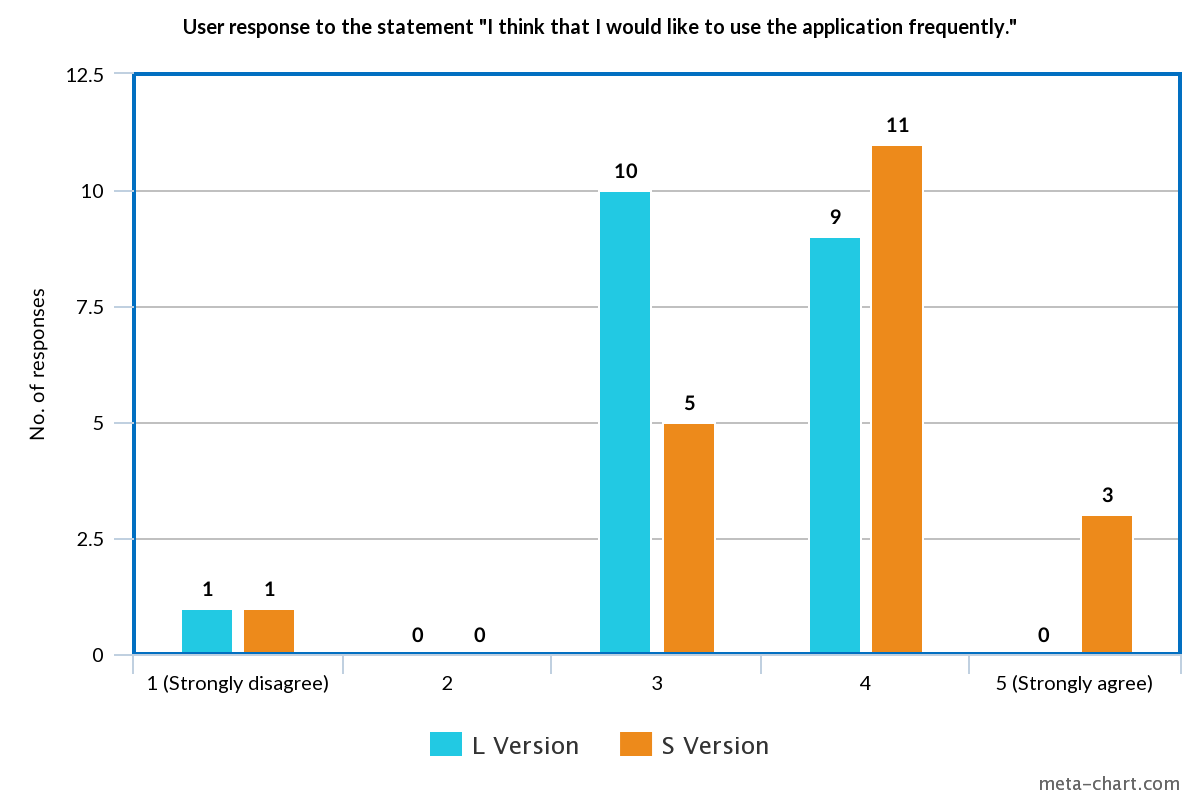
\includegraphics[width=85mm]{images/s1.png}
\caption{User response to the statement "I think that I would like to use the application frequently."}

\end{center}
\end{figure}

\begin{figure}[!ht]
\begin{center}

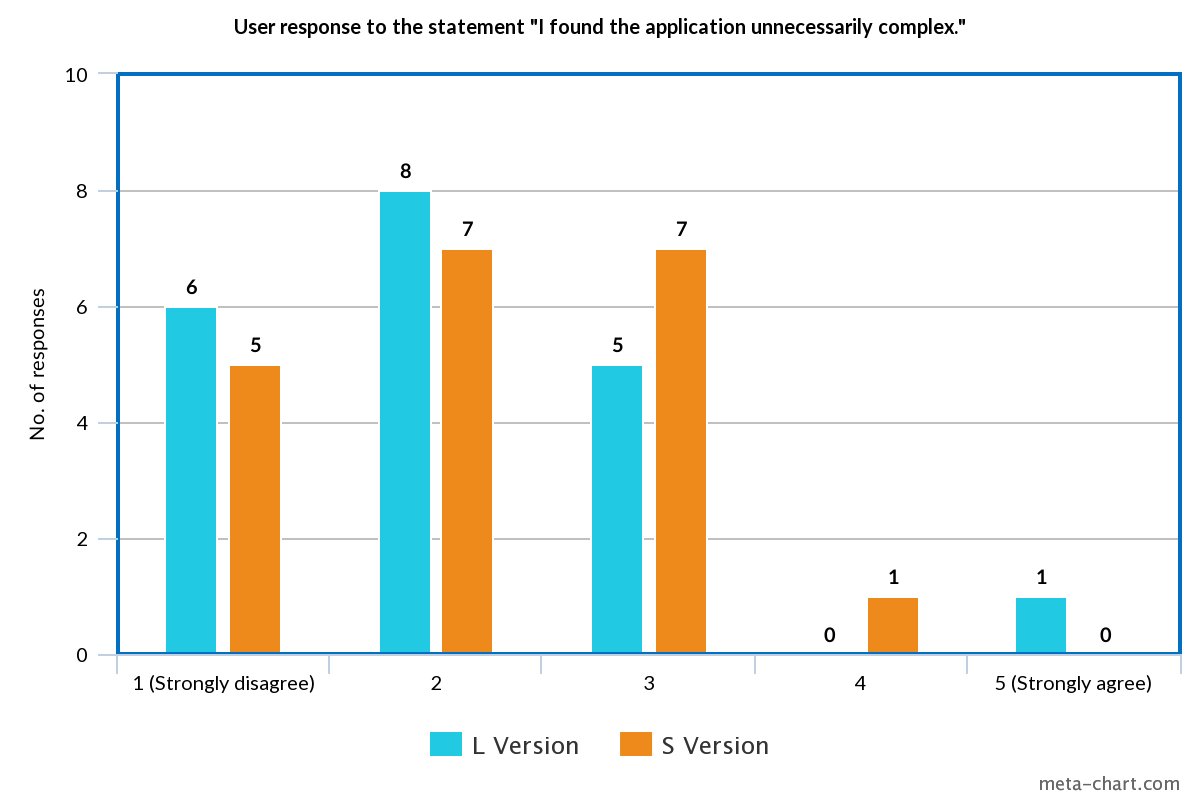
\includegraphics[width=85mm]{images/s2.png}
\caption{User response to the statement "I found the application unnecessarily complex."}

\end{center}
\end{figure}

\begin{figure}[!ht]
\begin{center}

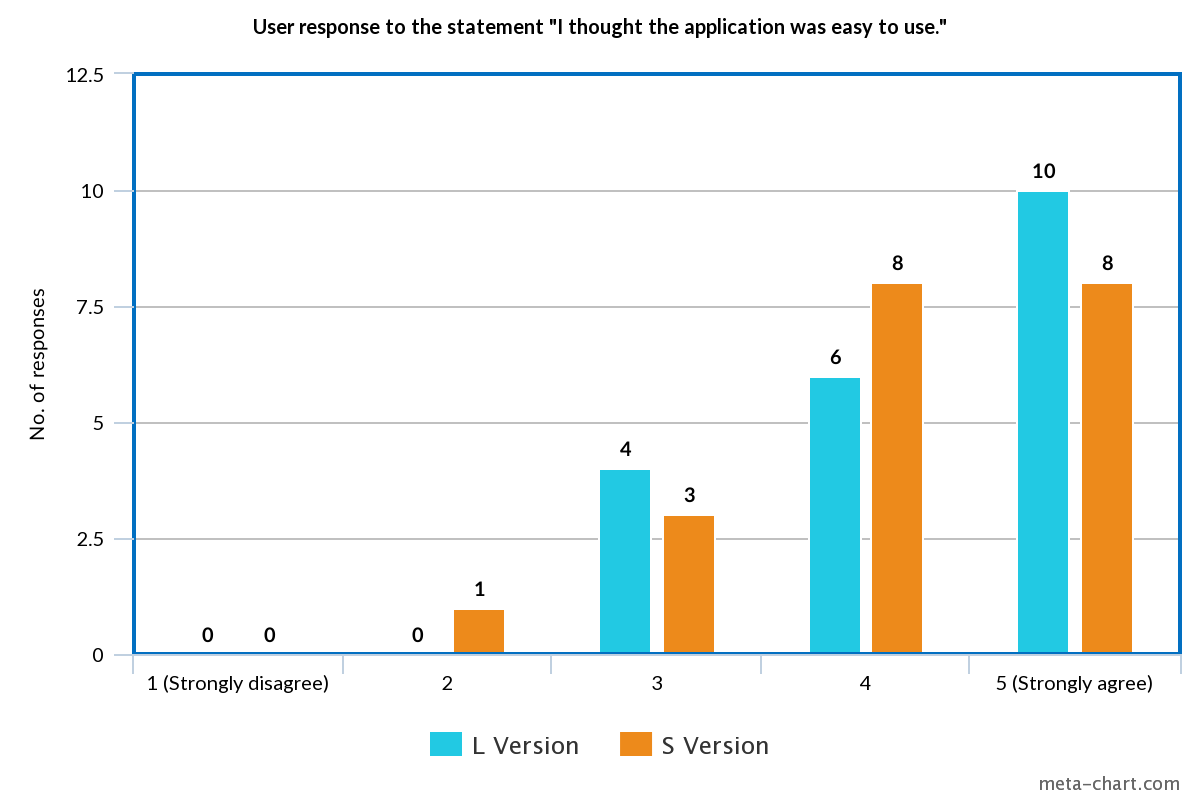
\includegraphics[width=85mm]{images/s3.png}
\caption{User response to the statement "I thought the application was easy to use."}

\end{center}
\end{figure}

\begin{figure}[!ht]
\begin{center}

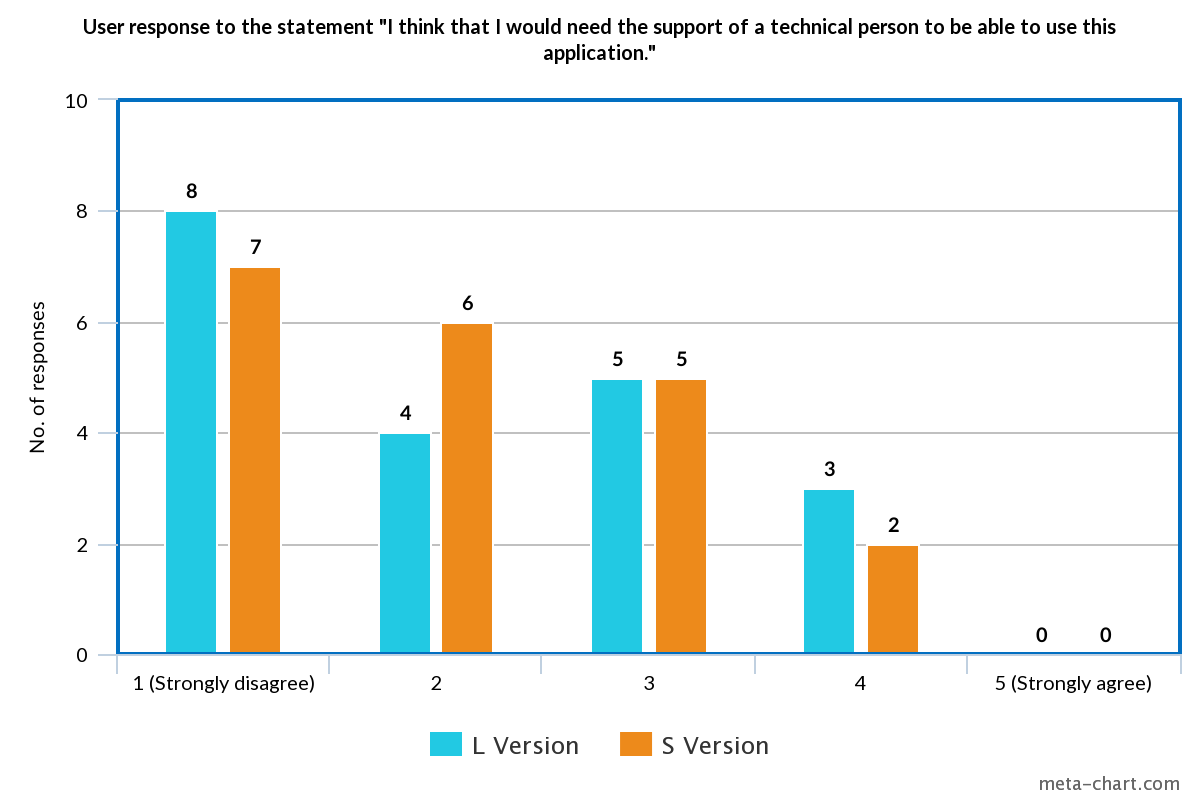
\includegraphics[width=85mm]{images/s4.png}
\caption{User response to the statement "I think that I would need the support of a technical person to be able to use this application."}

\end{center}
\end{figure}

\begin{figure}[!ht]
\begin{center}

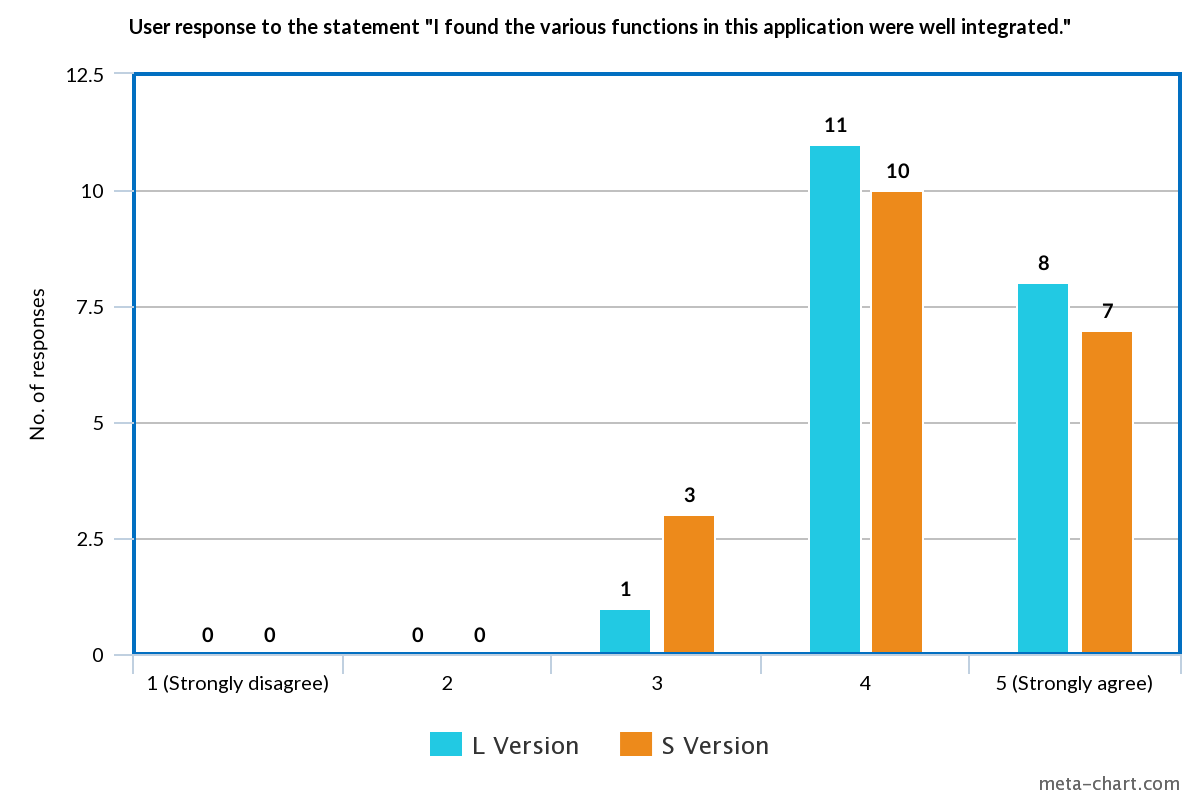
\includegraphics[width=85mm]{images/s5.png}
\caption{User response to the statement "I found the various functions in this application were well integrated."}

\end{center}
\end{figure}


\begin{figure}[!ht]
\begin{center}

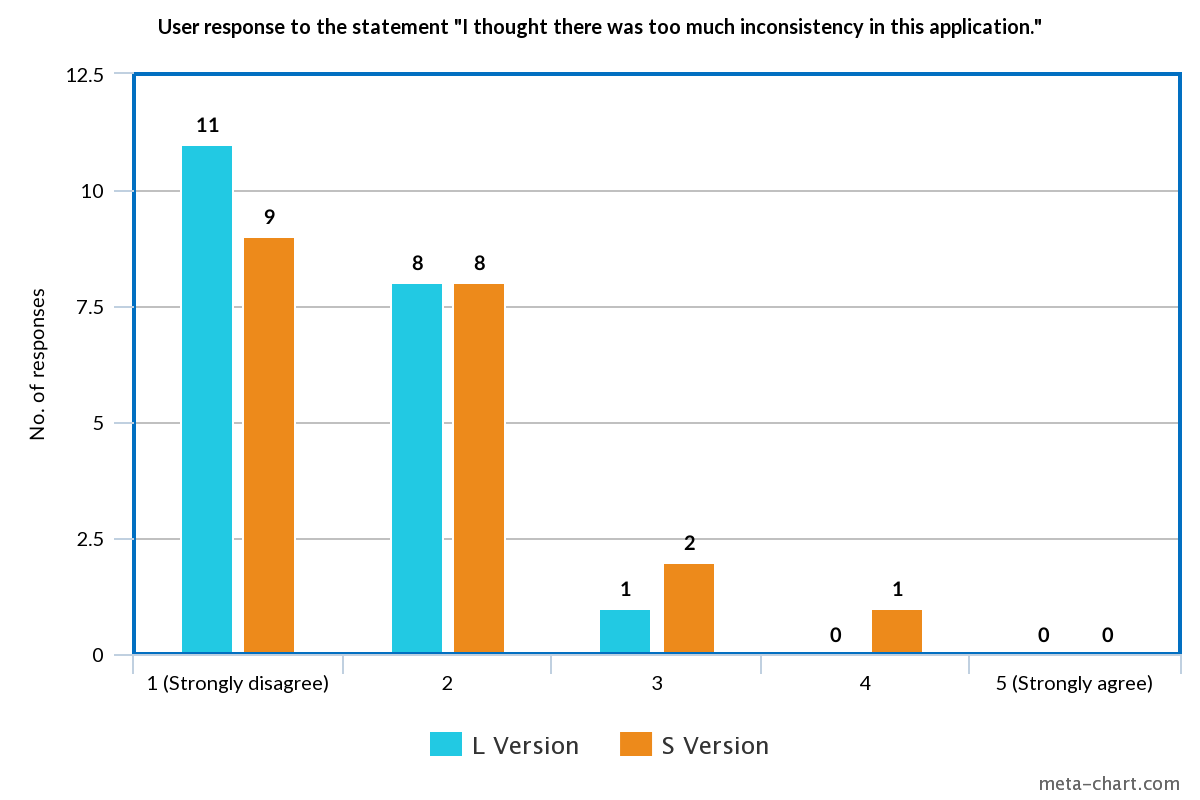
\includegraphics[width=85mm]{images/s6.png}
\caption{User response to the statement "I thought there was too much inconsistency in this application."}

\end{center}
\end{figure}

\begin{figure}[!ht]
\begin{center}

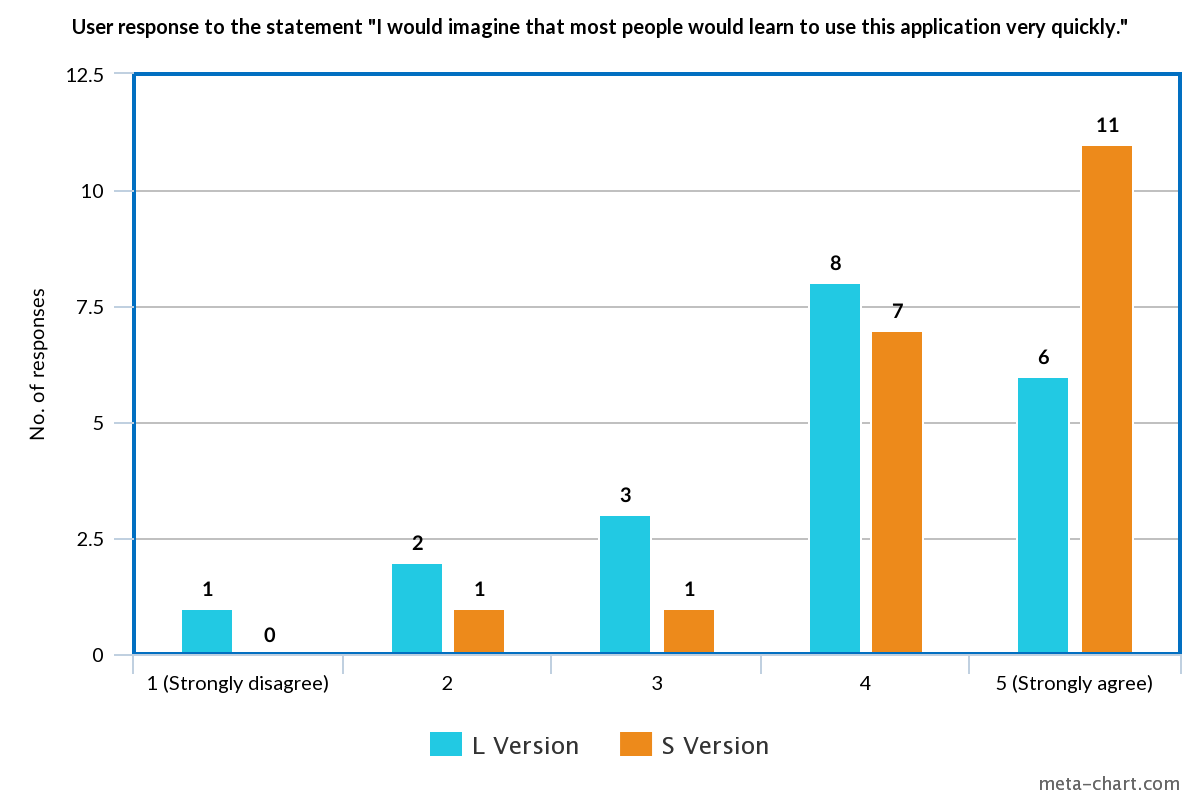
\includegraphics[width=85mm]{images/s7.png}
\caption{User response to the statement "I would imagine that most people would learn to use this application very quickly."}

\end{center}
\end{figure}

\begin{figure}[!ht]
\begin{center}

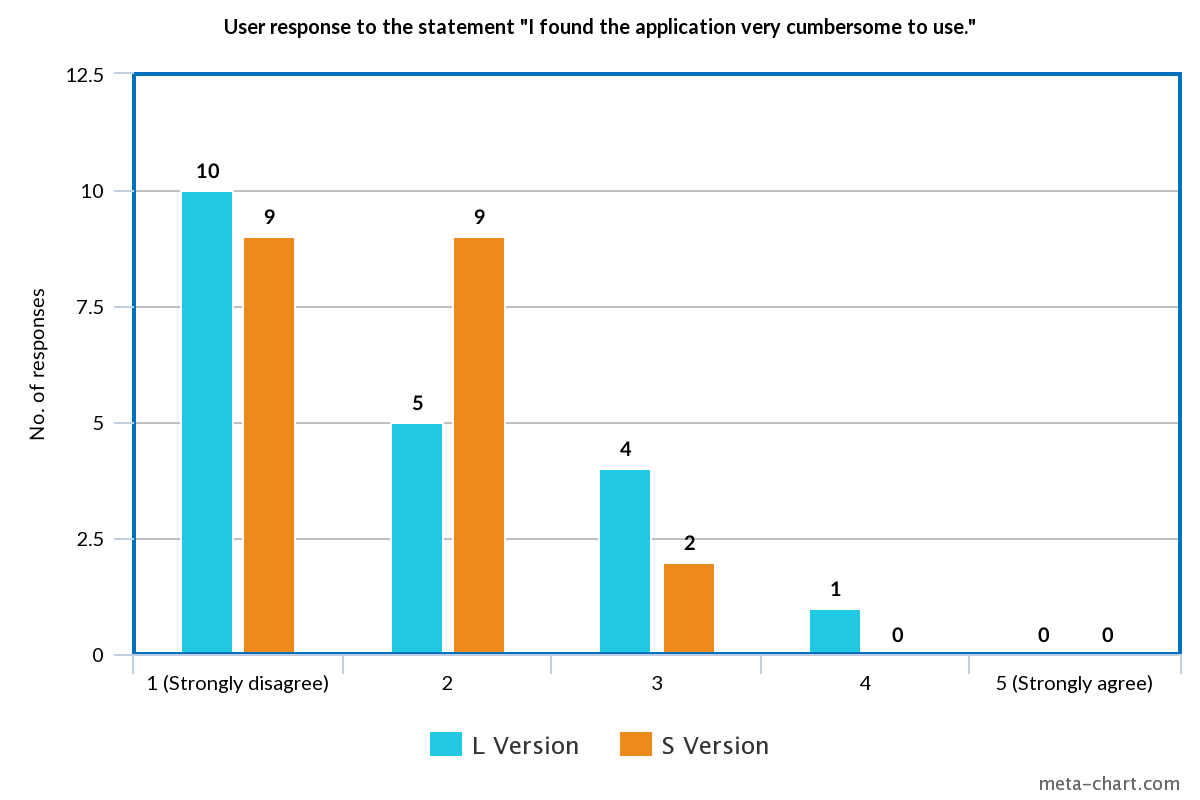
\includegraphics[width=85mm]{images/s8.png}
\caption{User response to the statement "I found the application very cumbersome to use."}

\end{center}
\end{figure}

\begin{figure}[!ht]
\begin{center}

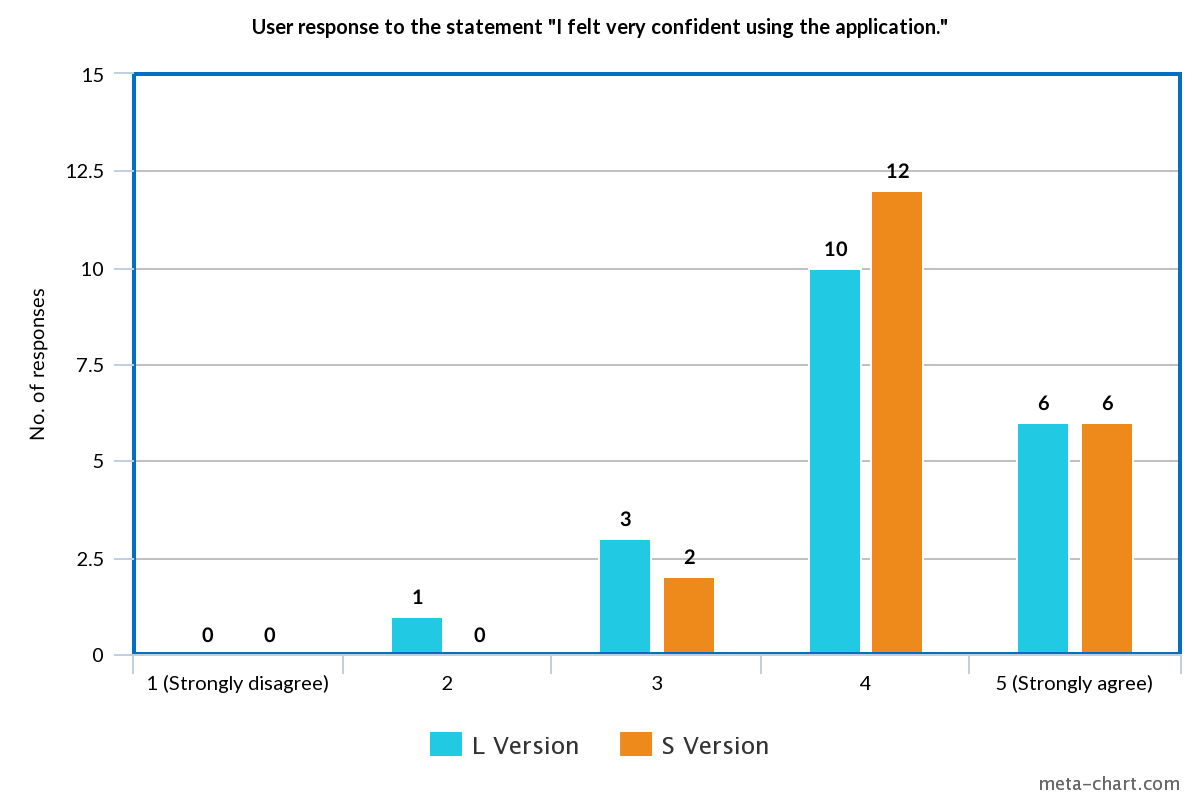
\includegraphics[width=85mm]{images/s9.png}
\caption{User response to the statement "I felt very confident using the application."}

\end{center}
\end{figure}

\begin{figure}[!ht]
\begin{center}

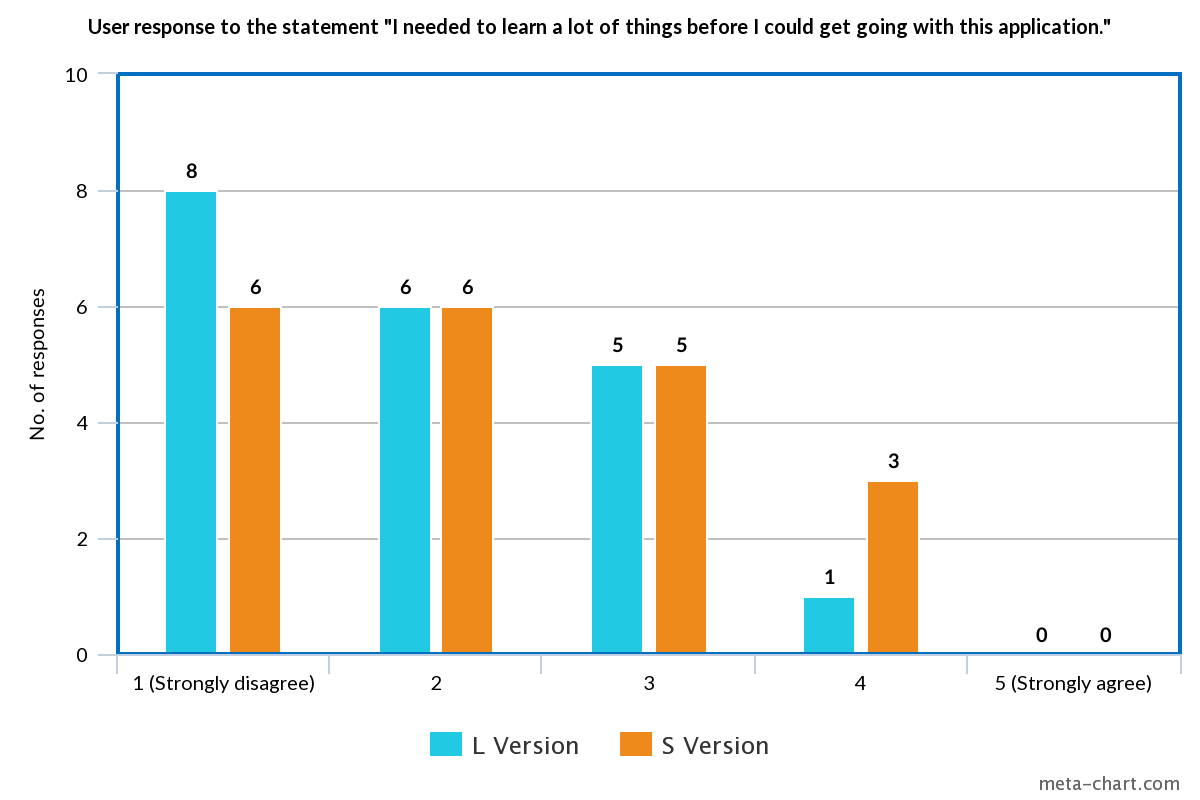
\includegraphics[width=85mm]{images/s10.png}
\caption{User response to the statement "I needed to learn a lot of things before I could get going with this application."}

\end{center}
\end{figure}

\begin{figure}[!ht]
\begin{center}

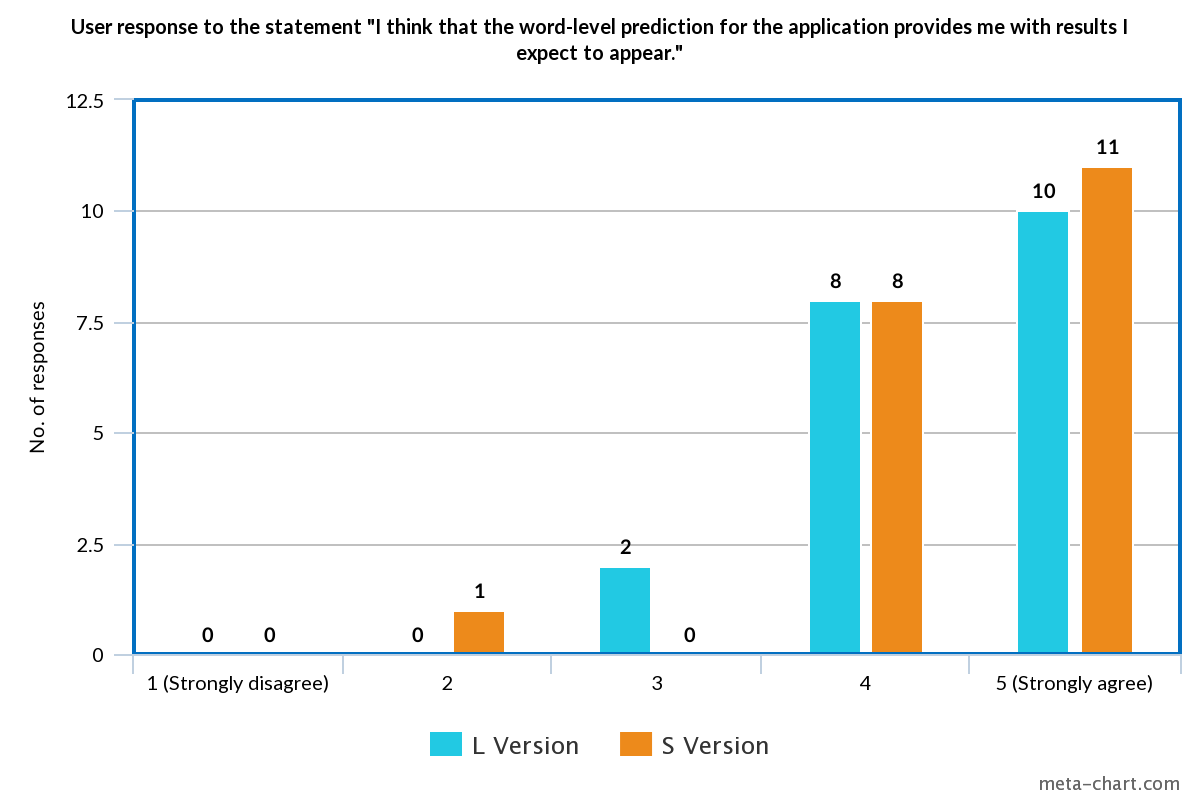
\includegraphics[width=85mm]{images/s11.png}
\caption{User response to the statement "I think that the word-level prediction for the application provides me with results I expect to appear."}

\end{center}
\end{figure}

\begin{figure}[!ht]
\begin{center}

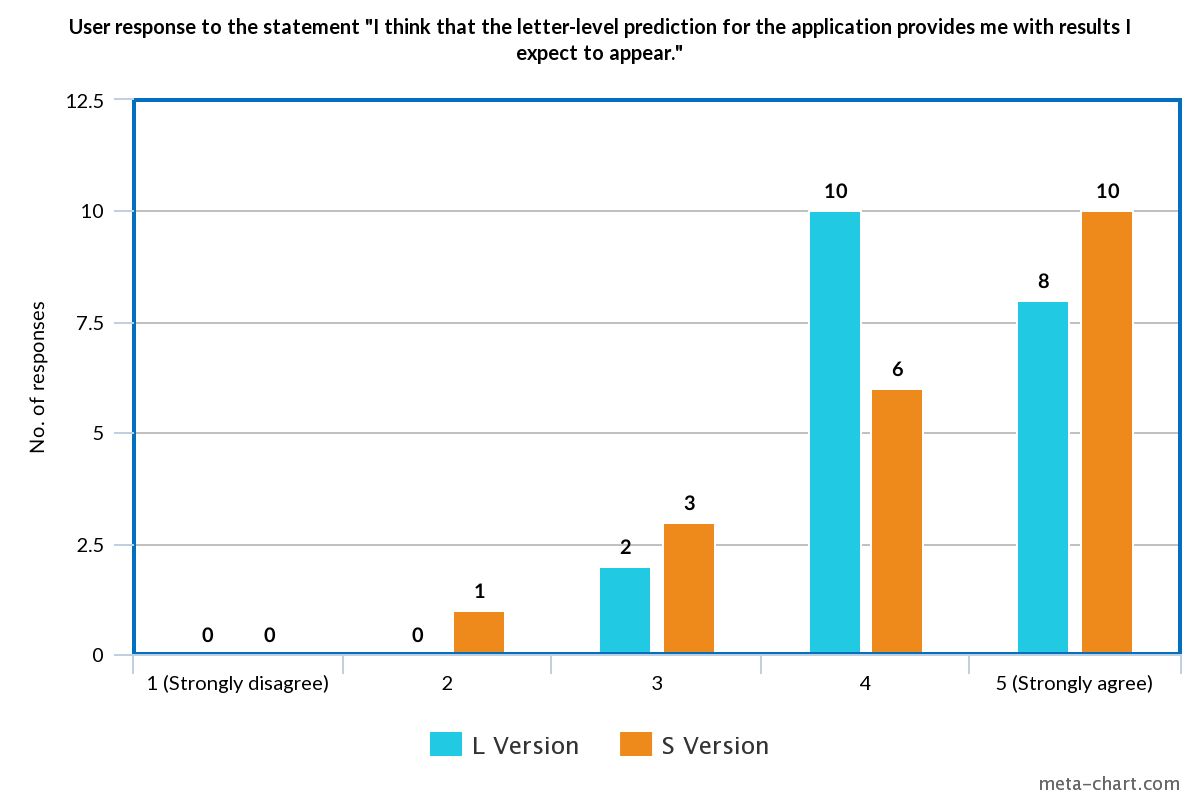
\includegraphics[width=85mm]{images/s12.png}
\caption{User response to the statement "I think that the letter-level prediction for the application provides me with results I expect to appear."}

\end{center}
\end{figure}

% BIBLIOGRAPHY
\bibliographystyle{./IEEE/IEEEtran}
\bibliography{./sayson-cs190-ieee}
\nocite{*}

% BIOGRAPHY
\begin{biography}
[{
\includegraphics{images/sayson.jpg}}]
{John Alvin L. Sayson} is an undergraduate student of the University of the Philippines Los Ba\~{n}os. He likes to spend the day sleeping, listening to music, playing music games and occasionally making music with his keyboard.
\end{biography}


\end{document}
 
